\subsection{Когомологии де Рама и компактные когомологии}

	\begin{definition} 
		Комплекс $\Omega^{\bullet}(\R^n)$ вместе с оператором $\mathrm{d}$ называется \emph{комплексом де Рама} на $\R^n$.

		Соответственно, когомологии этого комлпекса называют \emph{когомологиями Де Рама} $\R^n$:
		\[
			H^{q}_{\mathrm{dR}}(\R^n) = \ker\lr*{\mathrm{d} \colon \Omega^{q}((\R^n)) \to \Omega^{q + 1}(\R^n)}/\mathrm{Im}\lr*{ \mathrm{d} \colon \Omega^{q - 1}(\R^n) \to \Omega^{q}(\R^n)}. 
		\]
	\end{definition}

	\begin{remark}
		То, что это комплекс, гарантируется тем, что $\mathrm{d}^2 = 0$ (и, соотвественно, в связи с этим мы имеем $\ker{\mathrm{d}} \supset \Im{\mathrm{d}}$).
	\end{remark}


	\begin{remark}
		Видно $\ker{\mathrm{d}}$~--- это замкнутые формы, а образ $\mathrm{d}$~--- точные формы. 	
		Например, $f(x, y) \mathrm{d}x + g(x, y) \mathrm{d}y$ замкнута тогда и только тогда, когда 
		\[
			\frac{\partial f}{\partial y} - \frac{\partial g}{\partial x} = 0.
		\]
	\end{remark}

	Класс когомологий формы $\omega$ мы будем обозначать $[\omega]$. 

	\begin{remark}
		Всё то же самое можно делать для открытого $U \subset \R^n$ таким образом: 
		\[
			\Omega^{\bullet}(U) = C^{\infty}(U) \otimes_{\R} \Omega^{\bullet}(\R^n).
		\]
		Таким образом, мы можем говорить о когомологиях де-Рама $H^{q}_{\dR}(U)$ для любого открытого подмножества $\R^n$. 
	\end{remark}

	Заметим, что гладкое отображение $f\colon U \to V$, где $U, V$~--- открытые  подмножества $\R^n$, индуцирует отображение на формах 
	\[
		f^{*}\colon \Omega^{q}(V) \to \Omega^{q}(U), \ \omega \mapsto f^{*}(\omega),
	\]
	а так как дифференциал коммутирует с пуллбеком (т.е. $\mathrm{d} f^{*}(\omega) = f^{*}(\mathrm{d}\omega)$, $f^{*}$ даст нам цепное отображение $\Omega^{\bullet}(V) \to \Omega^{\bullet}(U)$:


	\begin{center}
		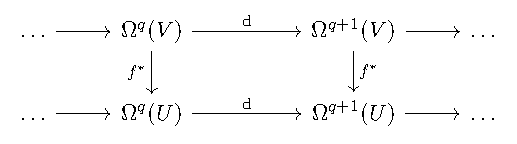
\includegraphics{lectures/7/pictures/cd_2.pdf}
	\end{center}

	\begin{definition} 
		\emph{Когомологии с компактным носителем} определяются следующим образом: рассмотрим комплекс дифференциальных форм с компактным носителем: 
		\[
			\Omega_{c}^{\bullet}(\R^n) \eqdef C^{\infty}_{0}(\R^n) \otimes_{\R} \Omega^{\bullet}(\R^n).
		\]
		Тогда когомологии с компактным носителем~--- это когомологии этого комплекса, мы будем обозначать их  $H^{q}_{c}(\R^n)$. 
	\end{definition}

	\begin{remark}
		Тут всё также корректно, так как $\mathrm{d}^2 = 0$. Но тут есть свои тонкости: нужно поступать аккуратнее с пуллбэком, так как пуллбэк формы с компактным носителем не обязан иметь компактный носитель. С другой стороны, если мы рассматриваем пулл-бэк при собственном отображении (т.е. таком, что прообраз компакта -- компакт), то всё выживает.  
	\end{remark}

	\begin{example}
		Вычислим $H^{\bullet}_{\dR}(\R)$.

		\begin{center}
			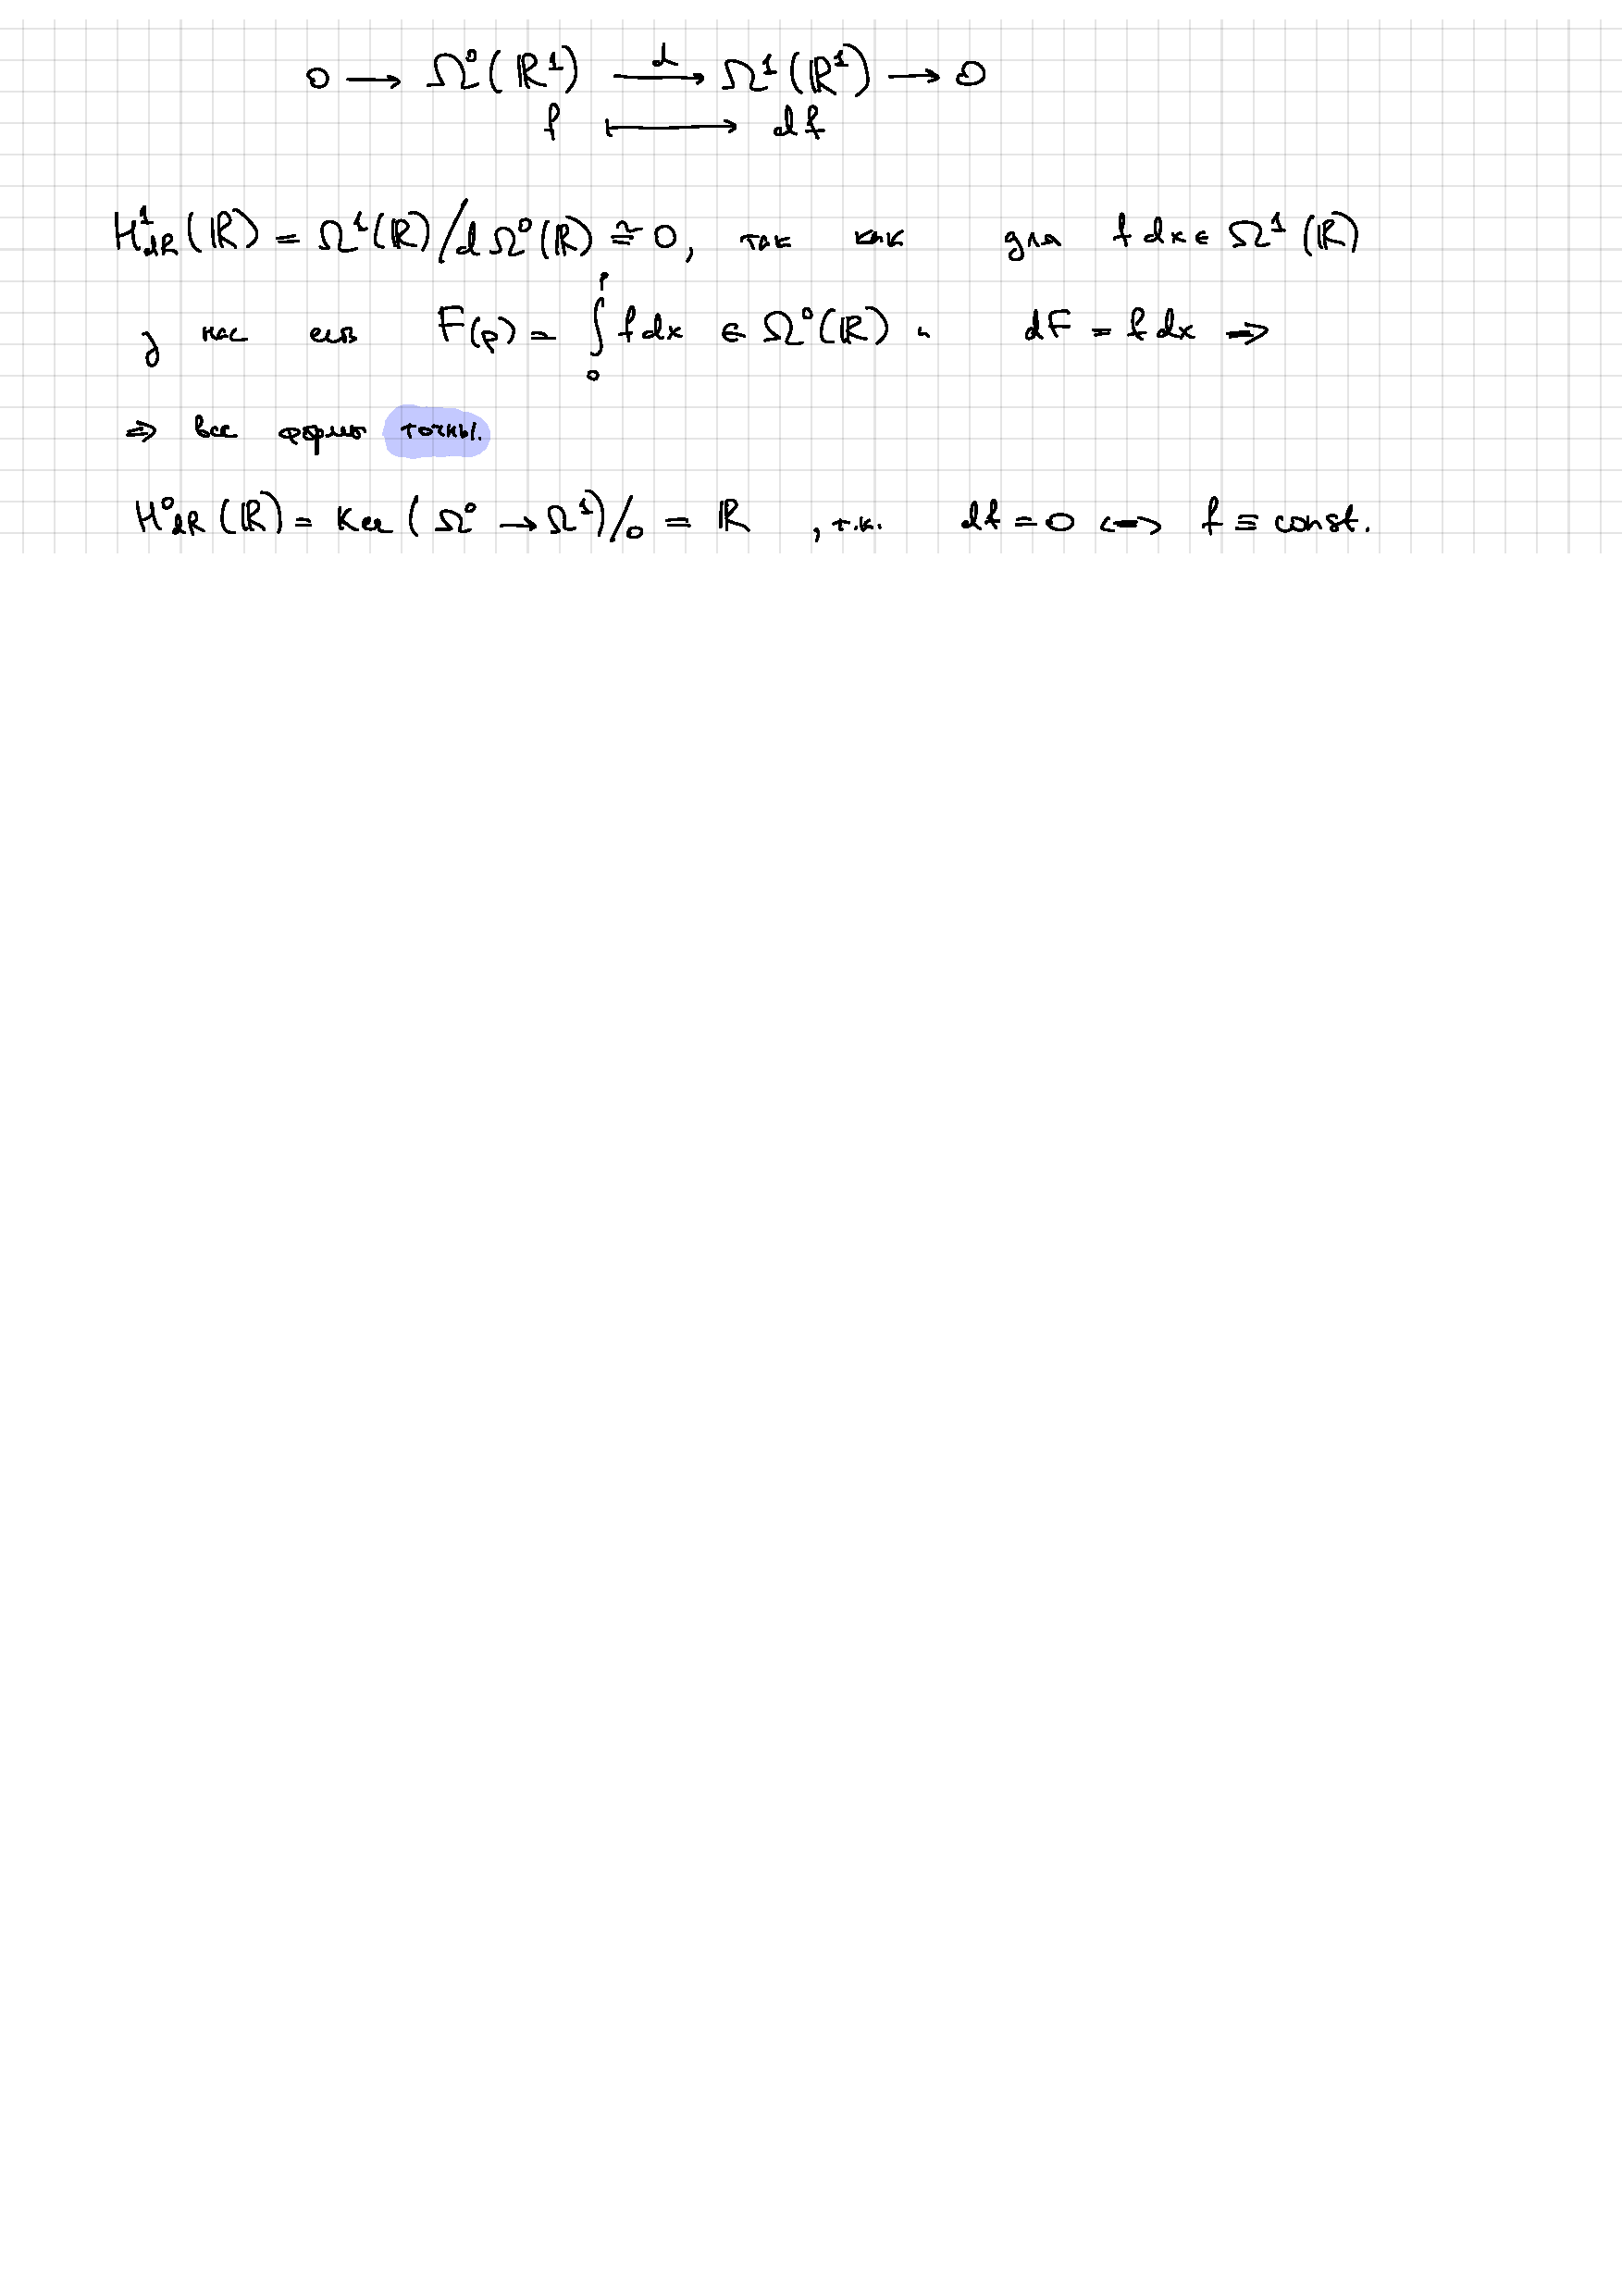
\includegraphics[scale = 0.6]{lectures/7/pictures/line_de_Rham.pdf}
		\end{center}

		Теперь вычислим компактные когомологии $H^{\bullet}_{c}(\R)$:
		\begin{center}
			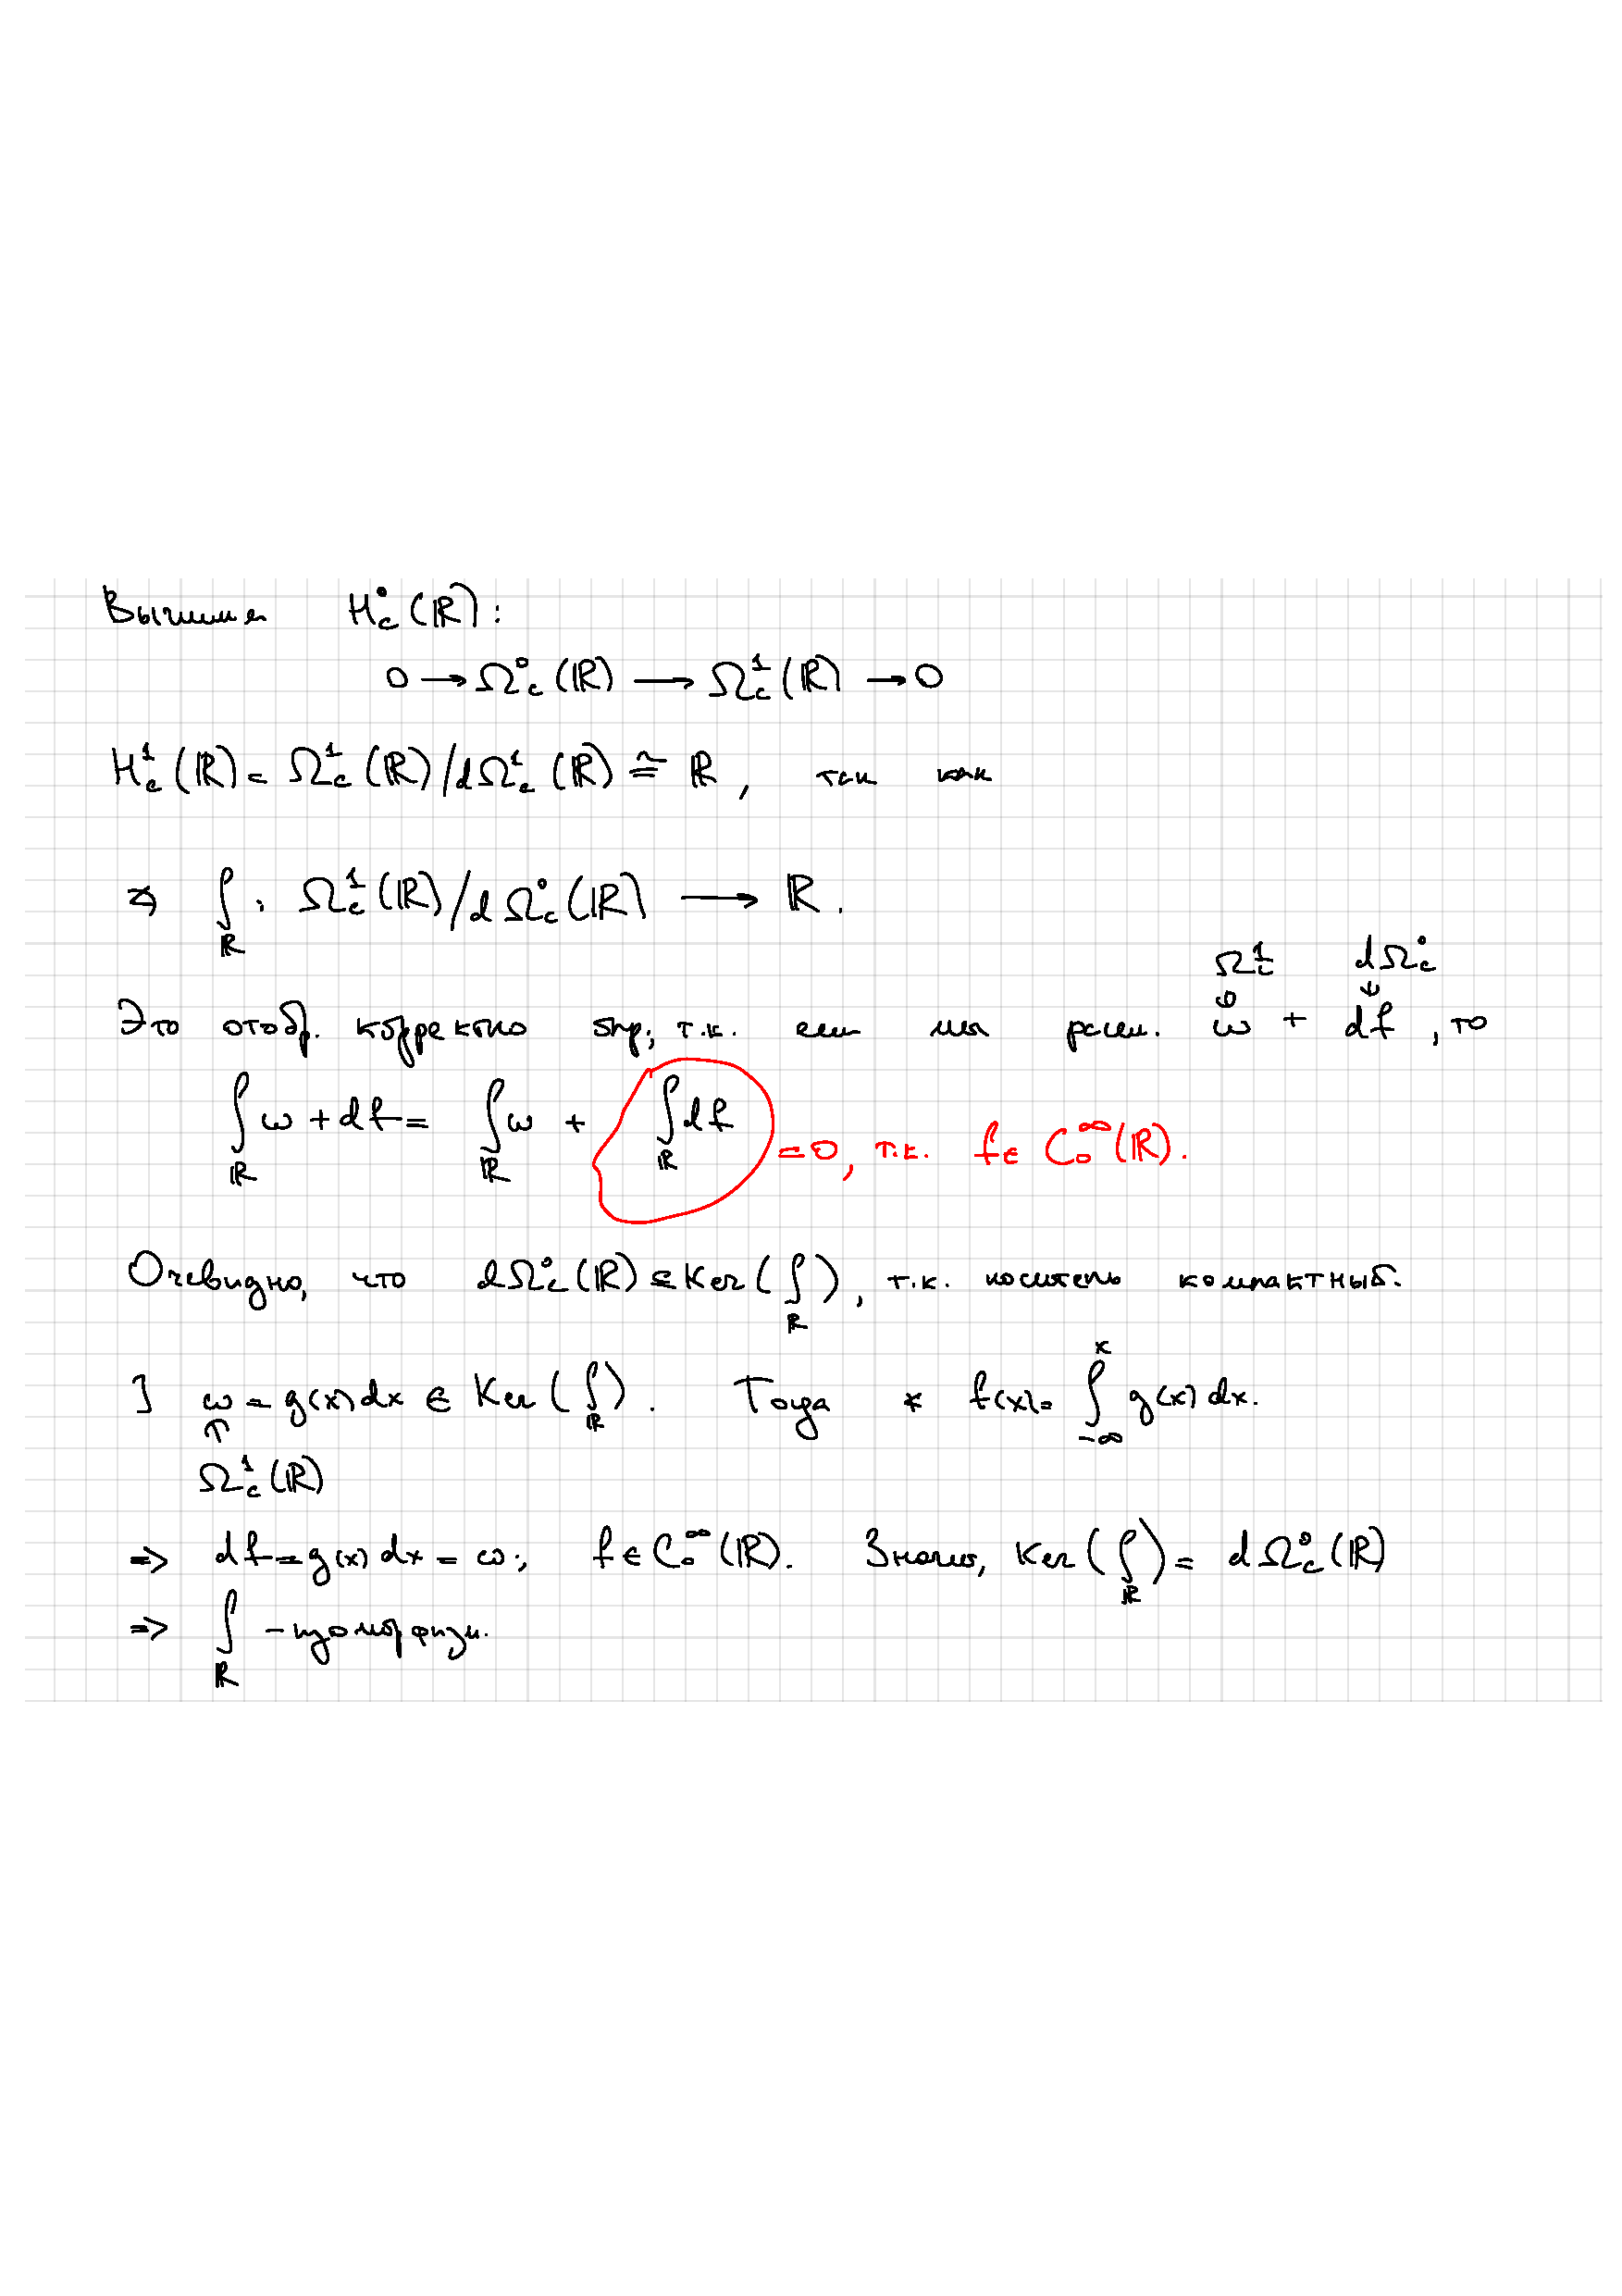
\includegraphics[scale = 0.6]{lectures/7/pictures/line_de_Rham_2.pdf}
		\end{center}

	\end{example}

	\subsection{Дифференциальные формы на многообразиях}

	На самом деле, тот факт, что гладкое отображение $f\colon U \to V$ индуцирует морфизм $f^* \colon \Omega^{\bullet}(V) \to \Omega^{\bullet}(U)$ (т.е., что дифференциал коммутирует с пуллбэком) на более изысканном языке означает, что $\Omega^*$ является контравариантным функтором из категории евклидовых пространств (и гладких отображений между ними) в категорию коммутативных дифференциальных градуированных алгебр. Коммутативность тут имеется в виду кососимметричная, то есть
	\[
		\tau \wedge \omega = (-1)^{\deg{\tau} \cdot \deg{\omega}} \omega \wedge \tau
	\]

	Более того, единственный такой функтор, совпадающий в нулевом члене с $C^{\infty}(\R^n)$~---  это как раз $\Omega^{\bullet}$.

	Действительно, из-за того, что $\Omega^{0}(\R^n) = C^{\infty}(\R^n)$, у нас сразу фиксирован базис из нужных $\mathrm{d}x_i$ (после того, как мы выбрали координатыне функции $x_i$), а дальше по линейности мы получаем всё те же 1-формы (и дальше по индукции). 
 

 	Этот функтор однозначно продолжается на категорию гладких многообразий. 

 	\begin{definition} 
 		Пусть $M$~--- гладкое многообразие, покрытое картами $\{ (U_{\alpha}, \varphi_{\alpha}) \}_{\alpha}$. Тогда дифференциальная форма $\omega$ на $M$ задаётся набором форм $\omega_{\alpha}$, каждая из которых задана в карте $U_{\alpha} \cong \R^n$, причём они согласованы на пересечении. 

 		Формальнее, у нас есть отображения 
 		\begin{center}
 			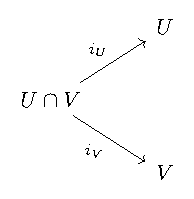
\includegraphics{lectures/7/pictures/cd_3.pdf}
 		\end{center}
 		и мы требуем, чтоб $i^*_{U} \omega_U = i^*_V \omega_V$ на $U \cap V$. 
 	\end{definition}

 	\begin{example}
 		Приведём несколько примером дифференциальных форм на многообразиях: 


 	\end{example}

 	\subsection{Точная последовательность Майера-Виеториса}

 	Начнём с напоминания про пуллбэк: если $f\colon M \to N$, причем в $M$ координаты $x_1, \ldots, x_m$,  а в $N$ координаты $y_1, \ldots, y_n$, то 
 	\[
 		f^{*}(\mathrm{d}y_i) = \sum_{j = 1}^n \frac{\partial y_i}{\partial x_j} \mathrm{d}x_j.
 	\] 

 	Тогда мы сможем считать и пуллбэки форм: 
 	\[
 		f^{*}(F(y_1, \ldots, y_n) \mathrm{d}y_1 \wedge \ldots \wedge \mathrm{d}y_k) = F(y_1(x_1, \ldots, x_m), \ldots) f^{*}(\mathrm{d}y_1) \wedge \ldots \wedge f^{*}(\mathrm{d}y_k).
 	\]

 	Но можно говорить и иначе (мы немного говорили про этот подход в первом параграфе). А именно, как мы помним, формы $\mathrm{d}y_i$ можно вычислять на касательных векоторах $\sum a_j \frac{\partial}{\partial y_j}$, как 
 	\[
 		\mathrm{d} y_i \lr*{\sum a_j \frac{\partial}{\partial y_j}} = a_i. 
 	\]
 	Тогда $k$-формы у нас действуют на наборах из $k$ векторов (как элемент $\Lambda^k T^*M$).

 	Пусть $f_* = \mathrm{d}f\colon TM \to TN$, тогда 
 	\[
 	 	f_*\lr*{\frac{\partial}{\partial x_j}} = \lr*{ \frac{\partial y_1}{\partial x_j}, \ldots, \frac{\partial y_n}{\partial x_j} }. 
 	 \] 
 	 Соответственно, пуллбэк  $f^*(\omega)$ мы тогда можем определить, как $k$-форму, действующую на наборах из $k$ векторов следующим образом: 
 	 \[
 	 	f^*(\omega)(v_1, \ldots, v_k) \eqdef \omega(f_*v_1, \ldots, f_* v_k). 
 	 \]
 	 Проверим, что для 1-форм это определение совпадает с предыдущим: 
 	 \[
 	 	f^*(\mathrm{d}y_i) = \sum a_j \mathrm{d}x_j, \quad a_j = \mathrm{d}y_i\lr*{f_* \frac{\partial}{\partial x_j}} = \mathrm{d}y_i\lr*{ \frac{\partial y_1}{\partial x_j}, \ldots, \frac{\partial y_n}{\partial x_j} } = \frac{\partial y_i}{\partial x_j},
 	 \]
 	  а этот коэффициент совпадает с тем, который был в предыдущем определении. Отсюда сразу следует, что это определение совпадает предыдущим и для  $k$-форм. 

 	  \begin{remark} 
 	  	Как мы уже отмечали, для форм с компактным носителем пулбэк определён только для собственных отображений. Зато определён \emph{пушфорвадр} (т.е. отображение в другую сторону) для открытых вложений (и, соответственно, пуллбэк для обратных отображений). Отсюда следует, в частности, что мы можем корректно (и так же как в обычном случае) определять формы с компактным носителем для многообразий. 
 	  \end{remark}

 	  Перейдём к \bf{точной последовательности Майера-Виеториса:}\\

 	  Пусть $M = U \cup V$, $U$  и $V$~--- открытые. Тогда у нас есть диаграммы: 

 	  \begin{center}
 	  	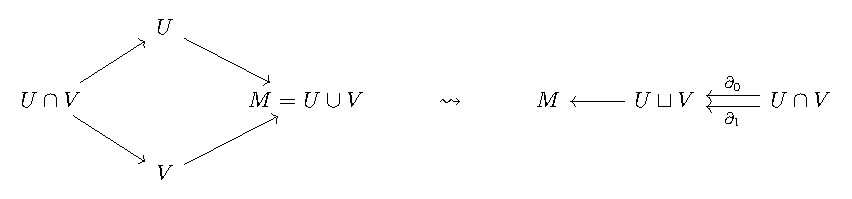
\includegraphics{lectures/7/pictures/cd_4.pdf}
 	  \end{center}

 	  Применяя функтор $\Omega^{\bullet}$, имеем 
 	  \begin{center}
 	  	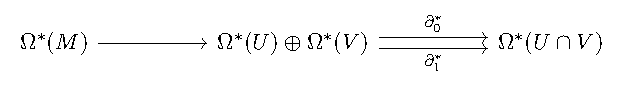
\includegraphics{lectures/7/pictures/cd_5.pdf}
 	  \end{center}

 	  \emph{Последовательностью Майера-Вьеториса} называется последовательность комплексов 
 	  \begin{center}
 	  		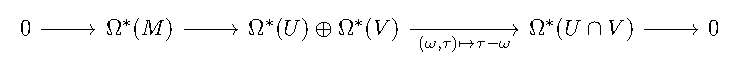
\includegraphics{lectures/7/pictures/cd_6.pdf}
 	  \end{center}

 	  \begin{remark}
 	  	Стрелка $\Omega^*(M) \to \Omega^*(U) \oplus \Omega^*(V)$~--- это сужение: $\omega \mapsto \omega\vert_U \oplus \omega\vert_{V}$. И, в следующей стрелке, когда мы берём разность, её мы тоже сужаем на $U \cap V$. 

 	  	Отметим, что под сужением на подмногообразие мы понимаем пулбек индуцированный вложением. 
 	  \end{remark}

 	  \begin{lemma} 
 	  	Последовательность Майера-Виеториса точна. 
 	  \end{lemma}
 	  \begin{proof}
 	  	Точность в первых двух членах очевидна (дольше писать, чем думать): 

 	  	 Проверим, что стрелка $\Omega^*(M) \to \Omega^*(U) \oplus \Omega^*(V)$ инъективна. Действительно, если $\omega\vert_{U} = 0$ и $\omega\vert_{V} = 0$, то $\omega = 0$ (так как $M = U \cup V$). 

 	  	 Теперь проверим точность в среднем члене. $\Ker\lr*{\Omega^*(U) \oplus \Omega^*(V) \to \Omega^*(U \cap V)} $~--- это формы $\tau \in \Omega^*(V)$ и $\omega \in \Omega^*(U)$, которые совпадают на $U \cap V$. Тогда просто по определению, так как формы согласованы на пересечении, из них можно склеить одну на $M$ (это доказывает включение $\Ker\lr*{\Omega^*(U) \oplus \Omega^*(V) \to \Omega^*(U \cap V)}  \subset \Im\lr*{ \Omega^*(M)  \to \Omega^*(U) \oplus \Omega^*(V)}$). С другой же стороны, если мы возьмём $\omega \in \Omega^*(M)$ и пройдём по двум стрелкам подряд, мы получим ноль: 
 	  	 \[
 	  	 	\omega \mapsto (\omega\vert_U, \omega\vert_V) \mapsto \lr*{\omega\vert_U - \omega\vert_V}\vert_{U \cap V} = \omega\vert_{U \cap V} - \omega\vert_{U \cap V} = 0. 
 	  	 \]
 	  	 Так мы получаем, что $\Im\lr*{ \Omega^*(M)  \to \Omega^*(U) \oplus \Omega^*(V)} \subset \Ker\lr*{\Omega^*(U) \oplus \Omega^*(V) \to \Omega^*(U \cap V)}$. 

 	  	 Теперь докажем точность в правом члене. Для этого воспользуемся разбиением единицы. 

 	  	 Докажем сначала для функций (для форм отсюда будет следовать афтоматически). Пусть $f \in \Omega^0(U \cap V)$, представим её в виде разности функций из $\Omega^0(U)$ и $\Omega^0(V)$. Пусть $\{ \rho_U, \rho_V \}$~--- разбиение единицы, подчиненное покрытию $\{ U, V \}$. Тогда мы определим $f_U = f \cdot \rho_V$, $f_V = - f \cdot \rho_U$. Тогда 
 	  	 \[
 	  	 	f \rho_V - (-f \rho_U) = f \cdot (\rho_U + \rho _V) = f \text{ на } U \cap V. 
 	  	 \]

 	  	 
 	  \end{proof}

 	  Теперь вспомним, что короткая точная последовательность комплексов индуцирует длинную точную последовательность когомологий. 

 	  \begin{center}
 	  		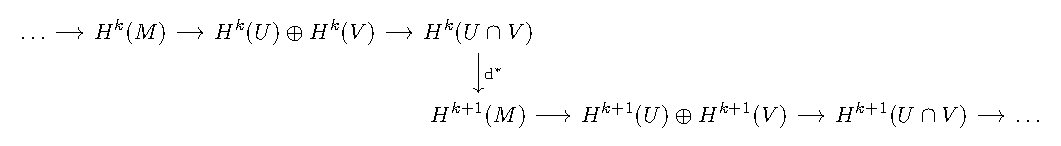
\includegraphics{lectures/7/pictures/cd_8.pdf}
 	  \end{center}

 	  Её также называют \bf{точной последовательностью Майера-Виеториса}. 

 	  Опишем явно, как выглядит связывающий кограничный гомоморфизм). Для этого нужно выполнить несложный диаграммный поиск. А именно, возьмём класс когомологий $[\omega] \in H^k(U \cap V)$ и выберем какого-то представителя $\omega \in \Omega^k(U \cap V)$. Отправим его наверх; так как это класс когомологий, $\mathrm{d}\omega = 0$. Теперь посмотрим из кого он пришёл и снова перейдём вверх. Так мы получим, что из пара форм $(\mathrm{d}(\rho_V \omega), - \mathrm{d}\rho_U \omega))$ согласована на пересечении и приходит из некоторой формы, которая и является $\mathrm{d}^*\omega$. 

 	  \begin{center}
 	  	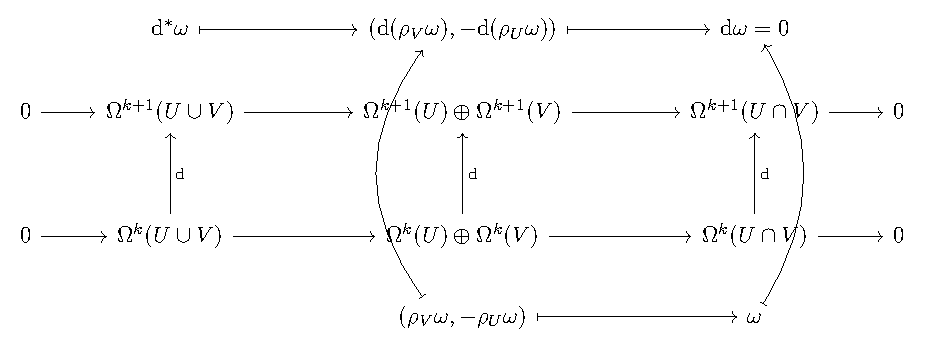
\includegraphics{lectures/7/pictures/cd_7.pdf}
 	  \end{center}

 	  Более того, слово <<некоторый>> тут исключительно в художественных целях, на самом то деле, как легко видеть из диаграммного поиска: 

 	  \[
 	  	\mathrm{d}^*[\omega] = \begin{cases} [-\mathrm{d}(\rho_V \omega)] \text{ на } U \\ [\mathrm{d}(\rho_U \omega)], \text{ на } V \end{cases}. 
 	  \]

	\noindent\bf{Последовательность Майера-Виеториса для форм с компактным носителем:}

	Напомним, что функтор $\Omega^{\bullet}_{c}(\_)$ удовлетворяет таким свойствам: 

	\begin{itemize}
		\item $\Omega^{\bullet}_{c}(\_)$ является контравариантным функтором относительно \emph{собственных отображений}. 

		\item $\Omega^{\bullet}_{c}(\_)$ является ковариантным функтором относительно \emph{открытых вложений}. 
	\end{itemize}


	В дальнейшем мы будем использовать именно ковариантную версию этого функтора. Тогда диаграмма 
	\begin{center}
		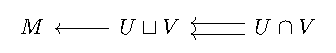
\includegraphics{lectures/7/pictures/cd_9.pdf}
	\end{center}
	индуцирует короткую точную последовательность комплексов 

	\begin{center}
		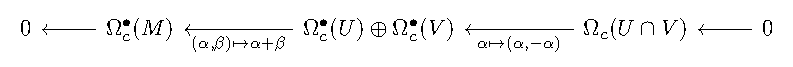
\includegraphics{lectures/7/pictures/cd_10.pdf}
	\end{center}

	\begin{lemma} 
		Последовательность Майера-Виеториса для форм с компактным носителем точна. 
	\end{lemma}
	\begin{proof}
		Здесь всё гораздо проще, чем в предыдущий раз. Обсудим точность в последнем члене. Гомоморфизм $\Omega^{\bullet}_{c}(M) \leftarrow \Omega_{c}^{\bullet}(U) \oplus \Omega_{c}^{\bullet}(V)$ сюръективен, так как прообразом формы $\omega$ является пара $(\rho_U \omega, \rho_V \omega)$ (где $\{ \rho_U, \rho_V \}$~--- разбиение единицы, подчинённое покрытию $\{ U, V \}$). 
	\end{proof}

	\begin{remark}
		Отметим, что в случае последовательности Майера-Виеториса для всех форм из формы на многообразии форму на кусочках мы получали так: 
		\[
			\omega \mapsto (\rho_V \omega, - \rho_U \omega).
		\]
		В то же время, в компактном случае мы поступаем несколько иначе 
		\[
			(\omega \rho_U, \omega\rho_V) \mapsto \omega. 
		\]
	\end{remark}
 	  
 	Тогда короткая точная последовательность комплексов индуцирует длинную точную последовательность когомологий (но, в другую сторону!)
 	\begin{center}
 		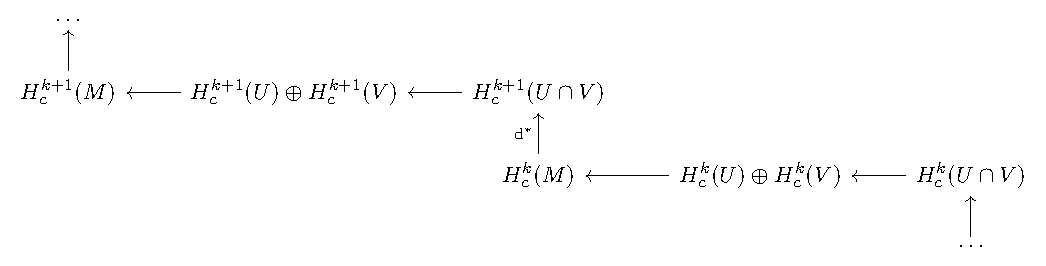
\includegraphics{lectures/7/pictures/cd_11.pdf}
 	\end{center}

 	\begin{example}
 		Переписать из книжки пример про окружность. 
 	\end{example}

 	
 	








